\section{Cross Product}

Cross Product also known as {\bf Vector Product} is a function denoted by
$$\times : \mathbb{E}^3 \times \mathbb{E}^3 \mapsto \mathbb{E}^3$$
i.e. it a binary operator on 2 vectors $\hat{t}$ returns a vector

\subsubsection{Motivation for Vector}
\vspace{-5px}
Given 2 non-zero vectors $\vec{u}$ and $\vec{v}$, construct a new vector say $\vec{w}$ such that it is {\bf orthoogonal} to {\em both} $\vec{u}$ and $\vec{v}$
\begin{figure}[ht]
	\centering
	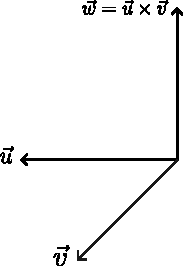
\includegraphics[scale=1.5]{cross_product.pdf}
	\caption{Cross Product}
	\label{fig:figure-9-cross-product}
\end{figure}

\begin{definition}
	Given 2 vectors $\vec{u}$ and $\vec{v} \in \mathbb{E}^3$, the {\bf cross product} of $\vec{u}$ and $\vec{v}$ is the vector $\vec{w}$ of {\bf length}
	\begin{equation}
		\label{eq:cross-product-length}
		\|\vec{w}\| = \|\vec{u}\|\|\vec{v}\|\sin\theta
	\end{equation}

	where $\theta$ is the {\bf planar angle between} $\vec{u}$ and $\vec{v}$ and {\bf direction} given by the {\bf right hand rule}
\end{definition}

We can determine the direction of $\vec{w}$ by using the {\bf right hand rule} as shown in Figure \ref{fig:figure-9-cross-product-direction}

\begin{figure}[ht]
	\centering
	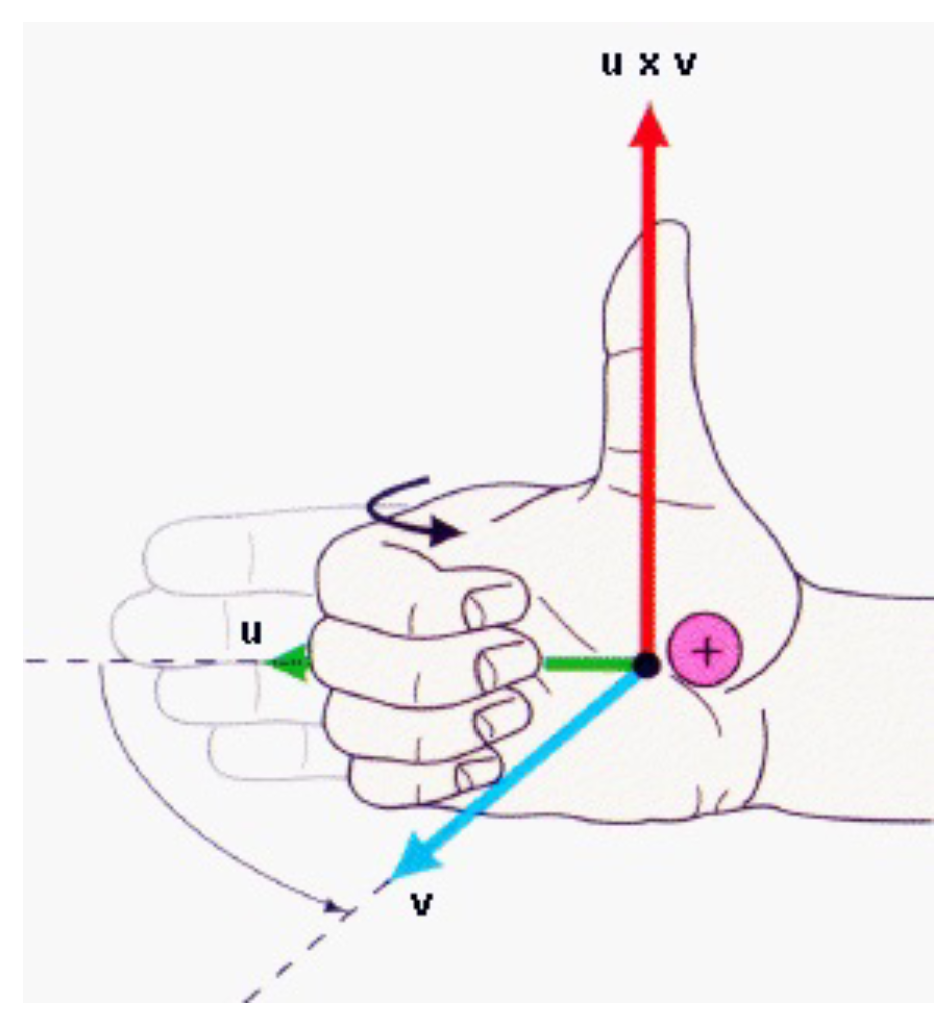
\includegraphics[scale=0.75]{right-hand-rule.png}
	\caption{Cross Product Direction}
	\label{fig:figure-9-cross-product-direction}
\end{figure}

\subsection{Properties of Scalar Product}
These properties can be seen as a consequence of the right and rule.
\begin{theorem}[Anti-Commutativity]
	Let $\vec{v}, \vec{w} \in \mathbb{E}^3$ Then
	\begin{equation}
		\label{eq:cross-product-anti-commutativity}
		\vec{v} \times \vec{w} = -(\vec{w} \times \vec{v})
	\end{equation}
\end{theorem}
\begin{figure}[ht]
	\centering
	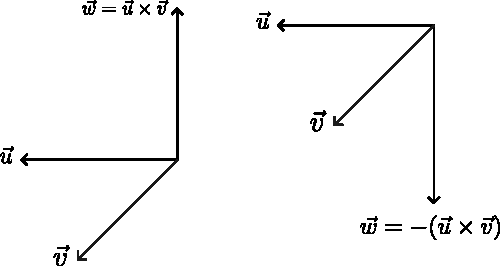
\includegraphics[scale=1]{anti-commutativity.pdf}
	\caption{Cross Product Anti-Commutativity}
	\label{fig:figure-9-cross-product-anti-commutativity}
\end{figure}

\begin{theorem}[Distributivity]
	Let $\vec{u}, \vec{v}, \vec{w} \in \mathbb{E}^3$ Then
	\begin{equation}
		\label{eq:cross-product-distributivity}
		\vec{u} \times (\vec{v} + \vec{w}) = (\vec{u} \times \vec{v}) + (\vec{u} \times \vec{w})
	\end{equation}
\end{theorem}

\begin{theorem}[Multiplication by Scalar]
	Let $\vec{u}, \vec{v} \in \mathbb{E}^3$ and $\lambda \in \mathbb{R}$ Then,
	\begin{equation}
		\label{eq:cross-product-multiplication-by-scalar}
		\lambda(\vec{u} \times \vec{v}) = (\lambda\vec{u}) \times \vec{v} = \vec{u} \times (\lambda\vec{v})
	\end{equation}
\end{theorem}

\begin{note}
	Properties of cross product on standard basis vectors
	\begin{align*}
		\hat{i} \times \hat{j} & = \hat{k}  \\
		\hat{j} \times \hat{k} & = \hat{i}  \\
		\hat{k} \times \hat{i} & = \hat{j}  \\
		\hat{j} \times \hat{i} & = -\hat{k} \\
		\hat{k} \times \hat{j} & = -\hat{i} \\
		\hat{i} \times \hat{k} & = -\hat{j} \\
	\end{align*}
\end{note}

\begin{note}
	The cross product is 0 when 2 vectors are {\bf parallel}. \\
	If $\vec{v} = \lambda \vec{u}$, then
	\begin{equation*}
		\begin{cases}
			0   \ \ \ \ \ \text{if } \lambda > 0 \\
			1 \ \ \ \ \ \text{if } \lambda < 0
		\end{cases}
	\end{equation*}
	Since $\sin 0 = \sin \pi = 0$, we get
	$$\mid \vec{u} \times \vec{v} \mid = \mid \vec{u} \mid \mid \vec{v} \mid\sin\theta = 0 $$
	And hence
	$$\vec{u} \times \vec{v} = 0 $$

	And therefore we can derive the following properties about standard basis vectors
	\begin{align*}
		\hat{i} \times \hat{i} & = 0 \\
		\hat{j} \times \hat{j} & = 0 \\
		\hat{k} \times \hat{k} & = 0 \\
	\end{align*}

\end{note}

\clearpage

\subsection{Co-Ordinate Version of Cross Product}

\begin{theorem}[Co-Ordinate formula for Cross Product]
	Let $\vec{u}, \vec{v}, \vec{w} \in \mathbb{E}^3$. Then
	\begin{equation}
		\label{eq:cross-product-formula}
		\vec{u} \times \vec{v} = (u_2v_3 - u_3v_2)\hat{i} + (u_3v_1 - u_1v_3)\hat{j} + (u_1v_2 - u_2v_1)\hat{k}
	\end{equation}
\end{theorem}
\begin{proof}
	Let $\vec{u}, \vec{v} \in \mathbb{E}^3$. Then
	\begin{flalign*}
		\vec{u} \times \vec{v} & = (u_1\hat{i} + u_2\hat{j} + u_3\hat{k}) \times (v_1\hat{i} + v_2\hat{j} + v_3\hat{k})                                                                                                                                    \\ \\
		                       & = (u_1\hat{i} \times v_1\hat{i}) + (u_1\hat{i} \times v_2\hat{j}) + (u_1\hat{i} \times v_3\hat{k}) + (u_2\hat{j} \times v_1\hat{i}) + (u_2\hat{j} \times v_2\hat{j}) + (u_2\hat{j} \times v_3\hat{k})                     \\ &+ (u_3\hat{k} \times v_1\hat{i}) + (u_3\hat{k} \times v_2\hat{j}) + (u_3\hat{k} \times v_3\hat{k}) \\ \\
		                       & = \cancel{u_1v_1 \hat{i} \times \hat{i}} + (u_1v_2 \hat{i} \times \hat{j}) + (u_1v_3 \hat{i} \times \hat{k}) + (u_2v_1 \hat{j} \times \hat{i}) + \cancel{u_2v_2 \hat{j} \times \hat{j}} + (u_2v_3 \hat{j} \times \hat{k}) \\ &+ (u_3v_1 \hat{k} \times \hat{i}) + (u_3v_2 \hat{k} \times \hat{j}) + \cancel{u_3v_3 \hat{k} \times \hat{k}} \\ \\
		                       & = (u_2v_3 - u_3v_2)\hat{i} + (u_3v_1 - u_1v_3)\hat{j} + (u_1v_2 - u_2v_1)\hat{k}
	\end{flalign*}
\end{proof}

\begin{note}
	We can also write the cross product as
	\begin{equation}
		\label{eq:cross-product-formula-2}
		\vec{u} \times \vec{v} = \begin{vmatrix}
			\hat{i} & \hat{j} & \hat{k} \\
			u_1     & u_2     & u_3     \\
			v_1     & v_2     & v_3     \\
		\end{vmatrix}
	\end{equation}
\end{note}

\begin{note}
	Showing that $\vec{u} \times \vec{v}$ is orthogonal to both $\vec{u}$ and $\vec{v}$
	\begin{align*}
		\vec{u} \cdot (\vec{u} \times \vec{v}) & = u_1(u_2v_3 - u_3v_2) + u_2(u_3v_1 - u_1v_3) + u_3(u_1v_2 - u_2v_1)    \\
		                                       & = u_1u_2v_3 - u_1u_3v_2 + u_2u_3v_1 - u_2u_1v_3 + u_3u_1v_2 - u_3u_2v_1 \\
		\Rightarrow \vec{u} \cdot (\vec{u} \times \vec{v}) = 0
	\end{align*}
	and hence orthogonal. Proof similat for the other one.
\end{note}
